%% =====================================================================
%% DP-FedBN — corrected IEEE conference manuscript.
%%
%% This is a faithful reconstruction of the source manuscript
%% ("When Does Federated BatchNorm Help under Differential Privacy?")
%% with the factual flaws identified during the thesis review fixed:
%%   (1) MIT-BIH class-imbalance statistic corrected to the true
%%       distribution (the rarest class is F at ~0.7%, not "Q ~0.07%").
%%   (2) FedPerf description corrected to the implemented rule
%%       (size/F1 convex combination, not a softmax of F1).
%%   (3) Central-test-set wording corrected (15% holdout for MIT-BIH;
%%       canonical fold 10 for PTB-XL).
%%   (4) Model architecture lists all five BatchNorm modules.
%%   (5) Figure captions match the actual figures (colours / panels).
%% Every numeric result is unchanged and matches results/metrics/*.csv.
%% See paper/README.md and ../Grad thesis files/thesis-draft/REVIEW-NOTES.md.
%% =====================================================================
\documentclass[conference]{IEEEtran}
\IEEEoverridecommandlockouts

\usepackage{cite}
\usepackage{amsmath,amssymb,amsfonts}
\usepackage{algorithm}
\usepackage{algorithmic}
\usepackage{graphicx}
\usepackage{booktabs}
\usepackage{multirow}
\usepackage{textcomp}
\usepackage{xcolor}
\usepackage[hidelinks]{hyperref}
\usepackage{url}

\graphicspath{{figures/}}

% Compact monospace for library / API names.
\newcommand{\code}[1]{\texttt{\small #1}}

\begin{document}

\title{When Does Federated BatchNorm Help under\\Differential Privacy? An Eval-Regime\\Characterization on Medical ECG Classification}

\author{
\IEEEauthorblockN{Efe Deniz Ba\u{g}lar}
\IEEEauthorblockA{Department of Computer Engineering\\
Ege University\\
\.{I}zmir, Turkey\\
efedenizbaglar45@gmail.com}
\and
\IEEEauthorblockN{Hasan Bulut}
\IEEEauthorblockA{Department of Computer Engineering\\
Ege University\\
\.{I}zmir, Turkey\\
hasan.bulut@ege.edu.tr}
}

\maketitle

\begin{abstract}
Federated learning (FL) for medical AI must reconcile two competing demands: per-site personalized performance and rigorous differential privacy (DP) guarantees. Federated BatchNorm (FedBN) achieves the former by keeping BatchNorm statistics local, but is incompatible with DP-SGD via standard libraries (Opacus), forcing most DP-FL deployments into BN-replacement workarounds (typically GroupNorm) that destroy the personalization mechanism. We formalize \emph{DP-FedBN}, a dual-optimizer composition that applies DP-SGD to non-BN parameters while keeping BatchNorm parameters and running statistics local. While the term ``DP-FedBN'' appears as a single-paragraph party-level DP baseline in~\cite{adcol} (Table~17, Laplace noise on aggregated model updates), to our knowledge this is the first \emph{record-level DP-SGD} composition of FedBN's BN-locality with explicit treatment of the Opacus engineering obstacle, and the first systematic medical empirical characterization across heterogeneity regimes and privacy budgets. We benchmark FedBN, DP-FedAvg+GroupNorm, and DP-FedBN on MIT-BIH 5-class beat classification and PTB-XL binary record classification across six non-IID partition regimes and three privacy budgets ($\sim$40 configurations). Two findings emerge. First, the \emph{eval-regime flip} is task-agnostic: FedBN's ranking inverts between pooled-central evaluation (where it loses by up to 0.31 macro F1) and per-client local evaluation (where it wins by up to $+0.72$), confirmed on both datasets. Second, DP-FedBN's local advantage is \emph{partition-dependent}: it preserves a $+0.17$ local-F1 edge on label-skew at $\varepsilon{=}3$, but loses to GroupNorm under Dirichlet skew on both datasets. We provide a heterogeneity-typed decision rubric for medical FL practitioners. All code and reproduction artifacts are released at \url{https://github.com/kanemoda/MedicalFL} (private during review).
\end{abstract}

\begin{IEEEkeywords}
Federated learning, differential privacy, batch normalization, ECG classification, non-IID data, Opacus, medical AI.
\end{IEEEkeywords}

\section{Introduction}
Federated learning (FL)~\cite{fedavg,rieke} is the canonical privacy-preserving paradigm for training deep models across distributed medical institutions without centralizing patient data. Each site trains locally and shares only model updates with a server. While this prevents raw-data exposure, the model updates themselves can leak private information~\cite{geyer}, motivating the use of differential privacy (DP)~\cite{abadi} on top of FL.

The standard recipe --- DP-SGD for the local optimizer plus size-weighted parameter aggregation --- works for many architectures, but breaks for one specific component: BatchNorm (BN)~\cite{batchnorm}. Per-sample gradients under BN are mathematically ill-defined because each sample's normalization depends on the batch mean and variance, which depend on the other samples in the batch. The Opacus library~\cite{opacus} enforces this constraint at initialization time: any \code{BatchNormNd} module triggers \code{UnsupportedModuleError}, halting privacy-engine setup before training can begin.

Opacus's recommended workaround replaces every BN layer with GroupNorm~\cite{groupnorm}, which computes per-sample channel-group statistics on the fly without running buffers. This is sound under DP, but architecturally lossy in the FL setting: it eliminates the very mechanism that FedBN~\cite{fedbn} relies upon for handling non-IID data. FedBN keeps client-specific BN statistics local --- never aggregated, never broadcast --- so each client's BN layers act as a learnable domain adapter for that client's data distribution. Under the standard GroupNorm fix, this mechanism is gone.

The space of reasonable solutions is small. One can pick utility (use FedBN, abandon DP), pick privacy at the cost of personalization (use DP-FedAvg with GroupNorm, abandon FedBN), or attempt to compose the two by selectively applying DP-SGD only to the parameters that actually leave the client. The third option is what we call DP-FedBN. The idea is straightforward in principle: since BN parameters and running statistics never cross the federation boundary in the FedBN protocol, they require no DP protection in the federated threat model; one only needs to ensure that the privacy engine sees and protects the non-BN parameters that \emph{do} cross the boundary. Implementing this in practice with off-the-shelf Opacus, however, requires a non-obvious freeze-then-unfreeze trick to bypass \code{ModuleValidator}, two parallel optimizers (one DP-protected, one plain), and careful coordination of state-dict layouts when the model is wrapped with \code{GradSampleModule}.

The term ``DP-FedBN'' has appeared in prior literature: in~\cite{adcol} (their Table~17 and Appendix~B.11), the authors include a one-paragraph ``DP-FedBN'' baseline implemented by clipping and adding Laplace noise to communicated model updates --- i.e., party-level DP in the sense of~\cite{geyer}. Our work differs in three concrete ways: (i) we apply DP-SGD at the \emph{record level} via per-sample gradient clipping, providing strictly stronger privacy guarantees than party-level Laplace mechanisms; (ii) we document the Opacus engineering obstacle (\code{ModuleValidator} rejection of \code{BatchNormNd}) and package a freeze-then-unfreeze workaround whose enabling discussion lives only in an Opacus GitHub issue~\cite{opacusissue} from 2022; (iii) we characterize DP-FedBN empirically on real medical tasks across multiple non-IID regimes and privacy budgets, rather than a single digit-recognition setting.

\emph{Contributions.} This paper makes three contributions, two empirical and one methodological:
\begin{enumerate}
\item \emph{Methodological --- record-level DP-SGD construction of DP-FedBN with engineering documentation.} We give a dual-optimizer construction that is compatible with off-the-shelf Opacus~1.5, document the implementation pitfalls (state-dict prefix mismatch when \code{GradSampleModule} wraps the model; ExpandedWeights' incompatibility with \code{BatchMemoryManager}), and validate that the construction passes Opacus's \code{ModuleValidator} without sacrificing FedBN's mechanism. Unlike the party-level Laplace baseline of~\cite{adcol}, our construction provides record-level $(\varepsilon,\delta)$-DP via DP-SGD per-sample gradient clipping.
\item \emph{Empirical~1 --- the eval-regime flip is task-agnostic.} On two datasets with substantially different tasks --- MIT-BIH 5-class beat-level classification and PTB-XL binary record-level classification --- and at matched non-IID partitions, FedBN ranks \emph{worst} on pooled-central evaluation while ranking \emph{best} on per-client local evaluation. The central-vs-local F1 gap reaches $+0.72$ on MIT-BIH label-skew ($C{=}2$). We argue that the eval-regime choice between pooled-central and per-client local evaluation matters more than method choice in many realistic deployment scenarios.
\item \emph{Empirical~2 --- DP-FedBN's local advantage is partition-dependent.} Under DP, the comparison between DP-FedBN and DP-FedAvg+GroupNorm is partition-sensitive: DP-FedBN preserves a $+0.17$ local-F1 edge on MIT-BIH label-skew at $\varepsilon{=}3$, but \emph{loses} on Dirichlet $\alpha{=}0.1$ on both datasets ($-0.008$ on MIT-BIH, $-0.234$ on PTB-XL $\varepsilon{=}3$). We give a mechanistic explanation --- DP noise on per-client BN parameters accumulates without the cross-client averaging that smooths it out for shared parameters --- and a decision rubric for practitioners.
\end{enumerate}

The rest of the paper is organized as follows. Section~\ref{sec:related} situates DP-FedBN against prior work. Section~\ref{sec:method} states the problem and describes the DP-FedBN construction. Section~\ref{sec:setup} details our experimental setup. Section~\ref{sec:results} presents the non-IID benchmark, the eval-regime finding, the privacy-utility frontier, and the cross-task replication. Section~\ref{sec:discussion} interprets the partition-dependent DP behavior and offers a practitioner rubric. Section~\ref{sec:conclusion} concludes with limitations and future work.

\section{Related Work}\label{sec:related}

\subsection{FL aggregation under non-IID data}
FedAvg~\cite{fedavg} is the standard FL algorithm: clients perform local SGD and the server averages model updates weighted by client sample counts. Under non-IID data --- where client distributions differ in covariate, label, or quantity, one of the central open problems of the field~\cite{kairouz} --- FedAvg drifts and under-converges. FedProx~\cite{fedprox} adds a proximal term that anchors each round's local optimum to the global broadcast, trading some local fit for stability. FedBN~\cite{fedbn} takes a different route: it leaves FedAvg's aggregation rule unchanged for Conv/Linear parameters but \emph{excludes} BN parameters and BN running statistics from aggregation entirely. Each client's BN layer thus calibrates to that client's data distribution, acting as a learned per-client domain adapter. FedBN was originally validated on feature-shifted partitions (DomainNet, Office-Caltech). Several extensions exist, including batch-specific BN with sharpness-aware minimization~\cite{tia} and personalized data transformations~\cite{privatefl}; we treat FedBN as our personalization baseline and do not deploy these extensions.

\subsection{Differential privacy in FL}
DP-SGD~\cite{abadi} provides $(\varepsilon,\delta)$-DP guarantees by clipping per-sample gradients to a bounded norm $C$ and adding calibrated Gaussian noise to the aggregated batch gradient. Its composition with FL is direct: each client runs DP-SGD locally, and the server's aggregation does not require additional DP because parameter updates are already DP-protected at the source~\cite{geyer}. The Opacus library~\cite{opacus} provides a PyTorch implementation including a \code{PrivacyEngine}, architectural compatibility checks (\code{ModuleValidator}), a privacy accountant, and helpers like \code{BatchMemoryManager} for memory-bounded per-sample gradient computation. We use Opacus~1.5 throughout.

\subsection{The BN--DP tension and existing workarounds}
The fundamental incompatibility is mechanical: BatchNorm couples samples within a batch through shared mean and variance statistics, making per-sample gradient clipping mathematically ill-defined. Opacus's \code{ModuleValidator} enforces this and rejects models containing \code{BatchNormNd} modules. The standard workaround, \code{ModuleValidator.fix()}, replaces every BN layer with GroupNorm~\cite{groupnorm}; GroupNorm computes per-sample channel-group statistics on the fly without running buffers, sidestepping the issue.

This workaround is, however, incompatible with FedBN's design. GroupNorm has no learnable running statistics, so there is no per-client state for FedBN's exclusion rule to keep local --- the mechanism that gives FedBN its non-IID advantage is gone. Two recent works address this gap differently. ResNetFed~\cite{resnetfed} modifies the network architecture globally to support DP federation, at the cost of replacing BN throughout. FedOnco-Bench~\cite{fedonco} provides a careful benchmark of medical FL under DP and non-IID conditions, but \emph{evaluates} FedBN and DP-SGD as competing alternatives, not as a combined method.

\subsection{Prior mentions of ``DP-FedBN''}
The term ``DP-FedBN'' appears in~\cite{adcol} (ADCOL, ICML 2023). Their Appendix~B.11 / Table~17 implements it as a one-paragraph baseline by clipping and adding Laplace noise to communicated model updates --- the party-level DP recipe of~\cite{geyer} --- evaluated on five digit datasets at $\varepsilon \in \{2,5,10\}$. Three differences distinguish our work: (i) \emph{privacy granularity}: we apply DP-SGD via per-sample gradient clipping (record-level DP), strictly stronger than the party-level Laplace mechanism; (ii) \emph{engineering}: we document the \code{ModuleValidator}-rejects-BN obstacle and package a freeze-then-unfreeze workaround discussed only in Opacus GitHub issue~\cite{opacusissue}; (iii) \emph{empirical scope}: two medical tasks, six non-IID regimes, three budgets ($\sim$40 configurations) versus a single label-balanced digit setting.

\subsection{Position of this work}
We contribute neither a new aggregation algorithm nor a new privacy mechanism. We contribute a record-level DP-SGD construction of FedBN+DP composition with documented Opacus engineering, and a multi-partition multi-budget medical evaluation (MIT-BIH+PTB-XL). The orthogonal axis we surface --- the eval-regime choice between pooled-central and per-client local evaluation --- is, we believe, of independent interest to the medical-FL benchmarking community.

\section{Method}\label{sec:method}

\subsection{Preliminaries: DP-SGD and the BN obstacle}
We assume a federated setting with $K$ clients indexed $k=1,\dots,K$. Each client owns a local dataset $\mathcal{D}_k$ of size $n_k = |\mathcal{D}_k|$. A global model $f_\theta$ with parameters $\theta$ is trained for $R$ rounds; in each round, every client receives the current global parameters $\theta_t$, performs $E$ epochs of local training on $\mathcal{D}_k$, and returns updated parameters $\theta_t^{(k)}$ to the server.

\emph{DP-SGD.}~\cite{abadi} modifies SGD by, at each step, computing per-sample gradients $g_i = \nabla_\theta \ell(f_\theta(x_i), y_i)$ for every sample $x_i$ in the minibatch $\mathcal{B}$, clipping each $g_i$ to a maximum $L_2$ norm $C$ via $\bar{g}_i = g_i \cdot \min(1, C/\lVert g_i \rVert_2)$, summing the clipped gradients, and adding Gaussian noise:
\begin{equation}
\hat{g} = \frac{1}{|\mathcal{B}|}\left( \sum_{i \in \mathcal{B}} \bar{g}_i + \mathcal{N}(0, \sigma^2 C^2 I) \right).
\label{eq:dpsgd}
\end{equation}
The noise multiplier $\sigma$ is chosen by an accountant so that the trained model satisfies an end-to-end $(\varepsilon,\delta)$-DP guarantee.

\emph{The BN obstacle.} Under BatchNorm with batch statistics $\mu_\mathcal{B}, \sigma_\mathcal{B}^2$, the output for sample $i$ is $\tilde{x}_i = (x_i - \mu_\mathcal{B})/\sqrt{\sigma_\mathcal{B}^2 + \epsilon_\mathrm{BN}}$, which depends on \emph{every} sample in $\mathcal{B}$ through $\mu_\mathcal{B}, \sigma_\mathcal{B}^2$. Consequently $g_i$ depends on samples $j \neq i$, and per-sample gradient clipping no longer bounds per-sample sensitivity. Opacus detects this and refuses to wrap any model containing \code{BatchNormNd} modules.

\emph{The standard workaround and its cost.} Opacus's recommended fix, \code{ModuleValidator.fix(model)}, replaces every BN layer with GroupNorm, which is privacy-safe but removes FedBN's per-client BN buffer mechanism (Section~\ref{sec:related}).

\subsection{FedBN aggregation}
FedBN~\cite{fedbn} modifies the aggregation rule, not the local training. Partition the model parameters as $\theta = (\theta^{\mathrm{BN}}, \theta^{\overline{\mathrm{BN}}})$, where $\theta^{\mathrm{BN}}$ collects all BN scale-shift parameters $(\gamma, \beta)$ and running buffers $(\mu, \sigma^2)$ across all BN layers. Then
\begin{equation}
\theta_{t+1}^{\overline{\mathrm{BN}}} = \sum_{k=1}^{K} \frac{n_k}{\sum_j n_j} \theta_t^{(k),\,\overline{\mathrm{BN}}}, \qquad
\theta_{t+1}^{(k),\,\mathrm{BN}} = \theta_t^{(k),\,\mathrm{BN}}.
\label{eq:fedbn}
\end{equation}
The BN parameters and buffers stay client-local; the rest is averaged as in FedAvg. Since the BN state never leaves the client, in the federated threat model it requires no DP protection.

\subsection{The DP-FedBN construction}
The challenge is implementational: Opacus's \code{ModuleValidator} checks the model architecture eagerly when \code{PrivacyEngine.make\_private\_with\_epsilon} is called, and refuses to wrap any model containing BN. We resolve this by \emph{temporarily freezing the BN parameters} so the validator treats them as inert (non-trainable) modules and proceeds.

\emph{Two-optimizer training step.} Each client constructs two optimizers:
\begin{itemize}
\item \code{opt$_A$}: an AdamW~\cite{adamw} optimizer over the non-BN parameters $\theta^{\overline{\mathrm{BN}}}$. This optimizer is wrapped by Opacus's \code{PrivacyEngine}, providing DP-SGD clipping and noise on the non-BN gradients only.
\item \code{opt$_B$}: a plain AdamW optimizer over the BN parameters $\theta^{\mathrm{BN}}$. This optimizer applies standard gradient updates without DP.
\end{itemize}
The BN running statistics $(\mu, \sigma^2)$ continue to update through their normal forward-pass exponential-moving-average path; they are not optimized parameters. The full client-side construction is given in Algorithm~\ref{alg:dpfedbn}.

\emph{Server side.} The server's aggregation rule is unchanged from FedBN, Eq.~\eqref{eq:fedbn}: average non-BN parameters across clients weighted by sample count, do not touch BN. The server never sees client BN state, so no DP composition is needed for it.

\begin{algorithm}[t]
\caption{DP-FedBN: client-side setup and one round}
\label{alg:dpfedbn}
\footnotesize
\begin{algorithmic}[1]
\REQUIRE Initial model $f_\theta$ with BN layers; train loader $\mathcal{L}_k$; target privacy budget $(\varepsilon,\delta)$; gradient clipping bound $C$.
\STATE \textbf{Round setup} (after global broadcast)
\STATE Receive $\theta_t^{\overline{\mathrm{BN}}}$; load into local model.
\FORALL{BN modules $m$}
  \STATE $m.\text{weight.requires\_grad} \leftarrow \text{False}$
  \STATE $m.\text{bias.requires\_grad} \leftarrow \text{False}$
\ENDFOR
\STATE Build $\text{opt}_A \leftarrow \mathrm{AdamW}(\theta^{\overline{\mathrm{BN}}})$
\STATE $(f_\theta, \text{opt}_A, \mathcal{L}_k) \leftarrow$ \code{make\_private\_with\_epsilon}($\dots$)
\FORALL{BN modules $m$}
  \STATE $m.\text{weight.requires\_grad} \leftarrow \text{True}$
  \STATE $m.\text{bias.requires\_grad} \leftarrow \text{True}$
\ENDFOR
\STATE Build $\text{opt}_B \leftarrow \mathrm{AdamW}(\theta^{\mathrm{BN}})$ (plain, no DP).
\STATE \textbf{Local training} (each minibatch $\mathcal{B}$)
\STATE $\text{opt}_A.\text{zero\_grad}()$; $\text{opt}_B.\text{zero\_grad}()$
\STATE $\hat{y} \leftarrow f_\theta(\mathcal{B}.x)$; $\ell \leftarrow \text{loss}(\hat{y}, \mathcal{B}.y)$
\STATE $\ell.\text{backward}()$
\STATE $\text{opt}_A.\text{step}()$ \quad $\triangleright$ DP-clipped + noised, on non-BN
\STATE $\text{opt}_B.\text{step}()$ \quad $\triangleright$ plain, on BN
\STATE \textbf{Round end}
\STATE Send $\theta^{\overline{\mathrm{BN}}}$ to server.
\STATE BN parameters and running stats remain local.
\end{algorithmic}
\end{algorithm}

\subsection{Threat model}
We adopt the standard FL threat model: an honest-but-curious server that respects the protocol but tries to infer client data from the parameter updates it sees, plus possibly malicious peer clients that observe broadcasts. Under DP-FedBN, the server and peers see only $\theta^{\overline{\mathrm{BN}}}$ updates, which are DP-protected via \code{opt$_A$} at every local step. The end-to-end privacy guarantee on $\theta^{\overline{\mathrm{BN}}}$ follows Opacus's privacy accountant applied per client. The BN state $\theta^{\mathrm{BN}}$ never crosses the federation boundary, so it requires no DP protection in this model.

If a stronger threat model is required --- for instance, where BN statistics could be inferred via repeated query attacks against a deployed personalized model --- additional protections on the deployed model would be needed. We do not address that scenario here and note it as a limitation.

\subsection{Implementation pitfalls}
Two pitfalls bit us during implementation and would bite a re-implementer the same way. (i)~When Opacus wraps a model, the underlying \code{GradSampleModule} prepends \code{\_module.} to all parameter and buffer keys in \code{state\_dict()}. Code paths that snapshot or restore client model state must consistently use the same unwrapping convention; we standardized on a \code{client.\_inner()} accessor and route every \code{state\_dict} interaction through it. (ii)~Opacus's alternative ExpandedWeights backend (\code{grad\_sample\_mode='ew'}) is incompatible with both \code{BatchMemoryManager}'s logical-batch chunking and \code{optimizer.zero\_grad(set\_to\_none=True)}; combining them crashes on the second optimizer step. We reverted to the default hooks-based backend, which paired with batch size 96 and \code{num\_workers=4} ran $\sim$6$\times$ faster than our initial configuration.

\section{Experimental Setup}\label{sec:setup}

\subsection{Datasets}
\emph{MIT-BIH Arrhythmia Database.} We use MIT-BIH~\cite{mitbih} for beat-level 5-class classification under the ANSI/AAMI EC57 standard~\cite{ec57,dechazal,mondejar}. Each beat is read on channel 0 (column 0 of the wfdb signal). R-peaks are taken from the standard \code{.atr} annotations; each beat is windowed as $\pm125$ samples around the R-peak (250 samples total, $\approx$694\,ms at 360\,Hz). Beats whose R-peak falls within 125 samples of either edge are dropped. Each beat is z-score-normalized within the window. The label follows the AAMI mapping: $\mathrm{N} = \{\mathrm{N,L,R,e,j}\}$; $\mathrm{S} = \{\mathrm{A,a,J,S}\}$; $\mathrm{V} = \{\mathrm{V,E}\}$; $\mathrm{F} = \{\mathrm{F}\}$; $\mathrm{Q} = \{/, \mathrm{f, Q}\}$. Non-beat annotations ($+$, $\sim$, $|$, \texttt{"}, etc.) are dropped rather than forced into Q. The four paced-record subjects (102, 104, 107, 217) are kept with their $/$ (paced) beats labelled Q, following EC57 and~\cite{dechazal}. Final dataset: \textbf{109\,453 beats across 48 records}, with class counts N 90\,595 ($\approx$82.8\%), Q 8\,040 ($\approx$7.3\%), V 7\,235 ($\approx$6.6\%), S 2\,781 ($\approx$2.5\%), and F 802 ($\approx$0.7\%).

\emph{PTB-XL.} We use PTB-XL~\cite{ptbxl}, the 100\,Hz \code{records100/} variant, for record-level binary classification (Normal vs Abnormal). Per record, the diagnostic superclass is the SCP code with the highest confidence whose \code{diagnostic\_class} is non-null in \code{scp\_statements.csv}; records with no such code are dropped. The binary task is NORM vs the union of $\{$MI, STTC, CD, HYP$\}$. Each record uses Lead~II only (column 1 of the 12-lead matrix), z-score-normalized, 1000 samples (10 seconds at 100\,Hz). Final dataset: \textbf{21\,388 records}, 9\,246 NORM and 12\,142 Abnormal. The canonical PTB-XL stratified folds are preserved; folds 1--9 enter client partitions and fold 10 is the central test set.

\emph{Why binary on PTB-XL.} We initially attempted PTB-XL 5-superclass classification on Lead~II. Three training regimes (44k-parameter model, 437k-parameter model with augmentation and stronger regularization, with cosine LR) all plateaued at test macro F1 $\approx 0.50$, with the HYP class stuck near 0.22. This was a representational bottleneck of single-lead input, not a capacity ceiling. We re-formulated PTB-XL as binary (NORM vs Abnormal), which is well-defined on Lead~II and reaches a balanced central macro F1 $\approx 0.81$. Multi-label PTB-XL with all 12 leads is a natural extension and is listed as future work (Section~\ref{sec:conclusion}).

\subsection{Federated setup}
All FL experiments use $K=5$ clients simulated via a custom sequential simulator (not Flower; we use a minimal in-process simulator to avoid IPC overhead during 100+ runs). The model is a 4-block 1D CNN with $\sim$437k parameters: Conv1D(64)\,--\,BN\,--\,Conv1D(128)\,--\,BN\,--\,Conv1D(256)\,--\,BN\,--\,Conv1D(256)\,--\,BN\,--\,FC(128)\,--\,BN\,--\,FC(num\_classes), ReLU activations, dropout 0.5 on the penultimate FC (five BatchNorm modules in total).

Each round runs $E=5$ local epochs of mini-batch SGD per client at batch size 96. Total rounds $R=30$ for DP runs and $R=50$ for non-DP runs. The optimizer is AdamW~\cite{adamw} with $\text{lr} = 1\times10^{-3}$ and weight decay $5\times10^{-4}$. The server aggregates after each round. For FedBN, BN parameters and buffers are excluded from aggregation per Eq.~\eqref{eq:fedbn}. FedPerf is a personalization-aware baseline that weights each client's update by an equal-weight ($\alpha{=}0.5$) convex combination of its $\ell_1$-normalized dataset size and its $\ell_1$-normalized local validation macro F1; we include it to contextualize FedBN but do not claim it as a contribution.

\subsection{Partition strategies}
We use six partition strategies on MIT-BIH:
\begin{itemize}
\item \textbf{IID}: stratified random split of beats across clients.
\item \textbf{Quantity skew} ($\beta{=}0.5$): client sizes follow a power law; smallest client has $\sim$0.5$\times$ the size of the median client.
\item \textbf{Dirichlet} $\alpha \in \{1.0, 0.5, 0.1\}$: each client's class distribution is drawn from a Dirichlet prior over the 5 classes; smaller $\alpha$ means greater label heterogeneity.
\item \textbf{Label skew} ($C{=}2$): each client owns exactly 2 of the 5 classes; this is the most extreme label heterogeneity available; each class appears in $\geq 1$ client.
\end{itemize}
For PTB-XL (binary), only IID, Dirichlet $\alpha{=}0.1$, and label skew $C{=}1$ are well-defined; the latter is the binary analogue of MIT-BIH's label-skew $C{=}2$ but produces degenerate single-class clients (Section~\ref{sec:results}-E). Partitions are seeded deterministically (\code{seed + client\_id}).

\subsection{Privacy configuration}
Privacy budgets: $\varepsilon \in \{1, 3, \infty\}$, $\delta = 10^{-5}$. Noise multiplier $\sigma$ is chosen by Opacus's \code{make\_private\_with\_epsilon} accountant per client at batch size 96. Gradient clipping bound $C = 1.0$; Opacus 1.5; default hooks-based backend (not ExpandedWeights, see Section~\ref{sec:method}). We compare three DP methods:
\begin{itemize}
\item \textbf{DP-FedAvg (raw BN)}: naive composition of DP-SGD with FedAvg on a BN-containing model. Expected to fail at finite $\varepsilon$ via Opacus's \code{ModuleValidator}.
\item \textbf{DP-FedAvg+GroupNorm}: FedAvg with all BN layers replaced by GroupNorm via \code{ModuleValidator.fix()}; this is the standard recommended workaround.
\item \textbf{DP-FedBN}: our dual-optimizer construction (Algorithm~\ref{alg:dpfedbn}) keeping BN local.
\end{itemize}

\subsection{Evaluation regimes}
We evaluate every run under \emph{two} regimes, since the choice of regime is itself a finding of this paper:
\begin{itemize}
\item \textbf{Central F1}: the final per-client model that is most representative (for FedAvg/FedProx/FedPerf, the global model; for FedBN, we report both client-1's model and the per-client average) is evaluated on a pooled held-out test set --- a 15\% stratified holdout for MIT-BIH and the canonical fold~10 for PTB-XL --- and we report macro F1.
\item \textbf{Local F1}: each client's final personalized model is evaluated on a per-client held-out validation slice (drawn from the same client's data); we report mean and standard deviation across clients.
\end{itemize}
Macro F1 is preferred over accuracy because the AAMI 5-class distribution on MIT-BIH is highly imbalanced (N $\approx$83\% versus the rarest class F $\approx$0.7\%); macro F1 weights all classes equally.

\subsection{Reproducibility}
All experiments use \code{seed=42}. \code{torch.backends.cudnn.deterministic = True}, all RNGs pinned, git SHA logged with each run. We accept \code{cudnn.benchmark = True} for the convolution kernel selection (non-deterministic across machines but stable on a given GPU/PyTorch combination); claims are reproducible on the same hardware. Hardware: GTX 1660 Super 6\,GB initially, RTX 4070 from the cross-task replication onward (PTB-XL phase). Code, configurations, and reproduction artifacts are released at the URL in the abstract.

\emph{Single-seed disclosure.} All numbers reported are single-seed realizations. Multi-seed variance quantification is the most important deferred experiment and is discussed as a limitation in Section~\ref{sec:conclusion}.

\section{Results}\label{sec:results}
We organize the results in four threads: (i) the centralized baselines that pin the upper bound; (ii) the non-IID benchmark on MIT-BIH and the eval-regime flip; (iii) the DP privacy-utility frontier on MIT-BIH; (iv) the cross-task replication on PTB-XL. Together they support the contributions of Section~\ref{sec:related}.

\subsection{Centralized baselines}
A single-machine centralized model on the full pooled training data achieves \textbf{macro F1 0.913} on MIT-BIH 5-class beats and \textbf{macro F1 0.813} on PTB-XL binary records. These numbers are the upper bound any FL configuration could approach; they pin ``IID-but-federated'' performance later in our results.

\subsection{Phase 1: Non-IID FL benchmark on MIT-BIH}
Table~\ref{tab:noniid} reports the best central F1 for each combination of partition $\times$ aggregation across 24 runs (6 partitions $\times$ 4 aggregations). Three patterns are visible.

\begin{table}[t]
\centering
\caption{MIT-BIH 5-class non-IID benchmark, best central macro F1 across 50 rounds (single seed). Higher is better. FedBN underperforms across every non-trivial partition.}
\label{tab:noniid}
\begin{tabular}{lcccc}
\toprule
Partition & FedAvg & FedProx & FedBN & FedPerf \\
\midrule
IID & \textbf{0.926} & 0.860 & 0.920 & \textbf{0.926} \\
Quantity skew & \textbf{0.922} & 0.884 & 0.912 & 0.913 \\
Dir. $\alpha{=}1.0$ & \textbf{0.937} & 0.889 & 0.911 & 0.928 \\
Dir. $\alpha{=}0.5$ & 0.926 & 0.903 & 0.850 & \textbf{0.928} \\
Dir. $\alpha{=}0.1$ & \textbf{0.745} & 0.735 & 0.554 & \textbf{0.745} \\
Label skew ($C{=}2$) & 0.527 & 0.386 & 0.219 & \textbf{0.530} \\
\bottomrule
\end{tabular}
\end{table}

First, IID-and-mild-skew partitions (IID, quantity skew, Dirichlet $\alpha \geq 0.5$) sit close to the centralized 0.913 ceiling for all four aggregations. Federation costs essentially nothing in this regime. Second, severe label heterogeneity (Dirichlet $\alpha{=}0.1$ and label skew $C{=}2$) collapses every aggregation, but FedBN collapses the most: on label skew $C{=}2$, FedBN reaches central F1 of only 0.219, while FedAvg, FedProx, and FedPerf reach 0.527, 0.386, and 0.530. This contradicts the original FedBN paper~\cite{fedbn}, which reported FedBN outperforming FedAvg on non-IID data. Third, FedProx at $\mu{=}0.01$ is consistently worse than FedAvg --- a known limitation of an un-tuned proximal term; tuning $\mu$ is future work.

\subsection{Phase 2: The eval-regime flip}
The FedBN collapse motivated a 7-check audit: BN-key partitioning, server-side BN exclusion, post-round BN divergence across clients, parameter-set integrity, IID parity, and a synthetic feature-shift sanity test reproducing the~\cite{fedbn} regime ($+0.45$ central F1 advantage for FedBN over FedAvg in the synthetic setup). The audit confirmed implementation correctness; the central-F1 collapse on real label-heterogeneous data is real, not a bug.

The audit's diagnostic check measured per-client local F1 alongside central F1 for the FedBN runs. The result, summarized in Table~\ref{tab:flip}, is the empirical core of this paper. FedBN's central F1 is 0.224 (the lowest of the four aggregations) while its local F1 is 0.942 (the highest of the four). The same model that ranks last under one evaluation regime ranks first under the other.

\begin{table}[t]
\centering
\caption{MIT-BIH label skew $C{=}2$ (most extreme partition): central macro F1 (pooled holdout) vs.\ per-client local macro F1 (mean $\pm$ std across 5 clients). FedBN ranks worst centrally and best locally, with a $+0.72$ flip.}
\label{tab:flip}
\begin{tabular}{lccc}
\toprule
Aggregation & Central F1 & Local F1 (mean$\pm$std) & $\Delta$ \\
\midrule
FedAvg & 0.527 & $0.823 \pm 0.178$ & $+0.297$ \\
FedProx & 0.386 & $0.488 \pm 0.380$ & $+0.101$ \\
\textbf{FedBN} & \textbf{0.224} & $\mathbf{0.942 \pm 0.053}$ & $\mathbf{+0.718}$ \\
FedPerf & 0.530 & $0.654 \pm 0.255$ & $+0.124$ \\
\bottomrule
\end{tabular}
\end{table}

\begin{figure*}[t]
\centering
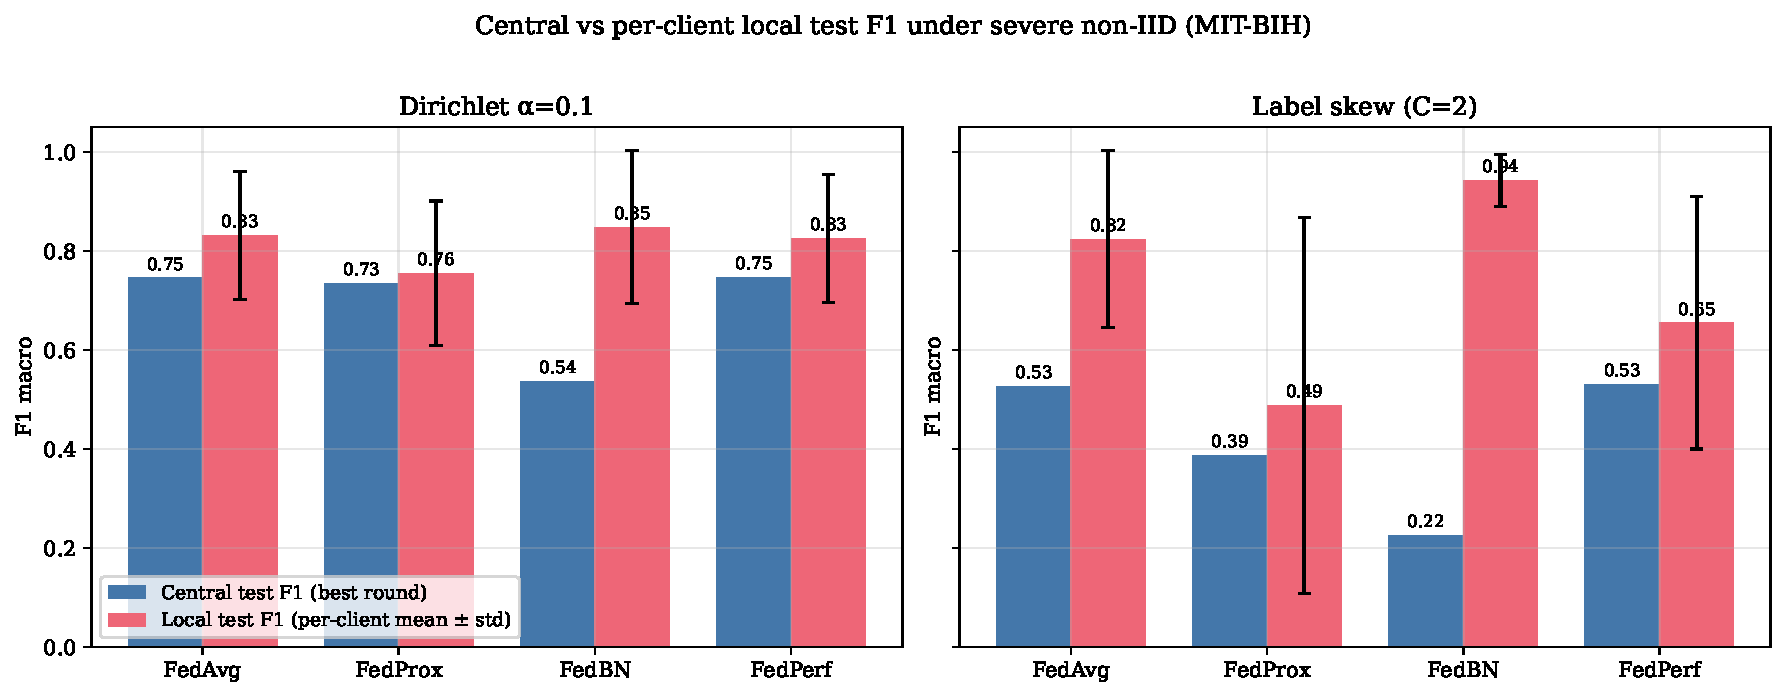
\includegraphics[width=0.95\textwidth]{fig_eval_regime.pdf}
\caption{Central vs.\ per-client local macro F1 across the four aggregations on MIT-BIH, for Dirichlet $\alpha{=}0.1$ (left) and label skew $C{=}2$ (right). Blue bars are central F1; red bars are local F1 (mean $\pm$ std). Under each partition FedBN has the lowest central F1 but the highest local F1 --- the eval-regime flip.}
\label{fig:flip}
\end{figure*}

\emph{Mechanism.} Each client's BN running statistics are calibrated to that client's local label distribution. Under label skew $C{=}2$, each client owns only 2 of the 5 classes, so its BN stats are tuned for those 2 classes. When that client's full model --- with its specialized BN --- classifies the central test set (which has all 5 classes in MIT-BIH proportions), BN normalization collapses on the classes the client never trained on. Per-client local evaluation, where each client only sees its own client's distribution, is fine. The same pattern holds on the milder Dirichlet $\alpha{=}0.1$ partition with smaller magnitude: FedBN central 0.536 vs.\ local $0.848 \pm 0.154$, a $+0.31$ flip; FedAvg central 0.745 vs.\ local $0.831 \pm 0.128$, a $+0.09$ flip. The sign and ordering are preserved; only the magnitude is smaller (Fig.~\ref{fig:flip}).

\subsection{Phase 3: DP privacy-utility frontier on MIT-BIH}
We run our three DP methods (raw FedAvg, DP-FedAvg+GroupNorm, DP-FedBN) across $\varepsilon \in \{1, 3, \infty\}$ on label skew $C{=}2$ and Dirichlet $\alpha{=}0.1$ --- the two most challenging partitions from Section~\ref{sec:results}-B. Table~\ref{tab:dp} reports the central and local F1 for each combination; achieved $\varepsilon$ values are within 0.5\% of target across all 7 finite-$\varepsilon$ runs. Three observations follow.

\begin{table}[t]
\centering
\caption{MIT-BIH DP privacy-utility benchmark (single seed, $\delta{=}10^{-5}$). Naive DP-FedAvg refused by Opacus at finite $\varepsilon$ --- the empirical motivation for DP-FedBN. On label skew, DP-FedBN keeps a $+0.17$ local-F1 advantage over DP-FedAvg+GN at $\varepsilon{=}3$; on Dirichlet the edge is mixed.}
\label{tab:dp}
\footnotesize
\setlength{\tabcolsep}{3pt}
\begin{tabular}{llcccc}
\toprule
Method & Partition & $\varepsilon$ & Ach.\ $\varepsilon$ & Cent.\ F1 & Local F1 \\
\midrule
DP-FedAvg (raw BN) & Lbl.\ $C{=}2$ & $\infty$ & --- & 0.517 & $0.829{\pm}0.192$ \\
DP-FedAvg (raw BN) & Lbl.\ $C{=}2$ & 3 & \multicolumn{3}{c}{REFUSED} \\
DP-FedAvg (raw BN) & Lbl.\ $C{=}2$ & 1 & \multicolumn{3}{c}{REFUSED} \\
DP-FedAvg+GN & Lbl.\ $C{=}2$ & $\infty$ & --- & 0.261 & $0.463{\pm}0.368$ \\
DP-FedAvg+GN & Lbl.\ $C{=}2$ & 3 & 2.996 & 0.191 & $0.295{\pm}0.241$ \\
DP-FedAvg+GN & Lbl.\ $C{=}2$ & 1 & 0.996 & 0.181 & $0.295{\pm}0.241$ \\
\textbf{DP-FedBN} & Lbl.\ $C{=}2$ & $\infty$ & --- & 0.221 & $\mathbf{0.937{\pm}0.043}$ \\
\textbf{DP-FedBN} & Lbl.\ $C{=}2$ & 3 & 2.993 & 0.181 & $\mathbf{0.467{\pm}0.264}$ \\
\textbf{DP-FedBN} & Lbl.\ $C{=}2$ & 1 & 0.996 & 0.217 & $\mathbf{0.344{\pm}0.194}$ \\
\midrule
DP-FedAvg (raw BN) & Dir.\ 0.1 & $\infty$ & --- & 0.738 & $0.816{\pm}0.130$ \\
DP-FedAvg (raw BN) & Dir.\ 0.1 & 3 & \multicolumn{3}{c}{REFUSED} \\
DP-FedAvg (raw BN) & Dir.\ 0.1 & 1 & \multicolumn{3}{c}{REFUSED} \\
DP-FedAvg+GN & Dir.\ 0.1 & $\infty$ & --- & 0.736 & $0.832{\pm}0.118$ \\
DP-FedAvg+GN & Dir.\ 0.1 & 3 & 2.996 & 0.382 & $0.376{\pm}0.101$ \\
DP-FedAvg+GN & Dir.\ 0.1 & 1 & 0.994 & 0.378 & $0.350{\pm}0.144$ \\
\textbf{DP-FedBN} & Dir.\ 0.1 & $\infty$ & --- & 0.551 & $0.861{\pm}0.130$ \\
\textbf{DP-FedBN} & Dir.\ 0.1 & 3 & 2.996 & 0.189 & $0.368{\pm}0.151$ \\
\textbf{DP-FedBN} & Dir.\ 0.1 & 1 & 0.994 & 0.251 & $0.465{\pm}0.308$ \\
\bottomrule
\end{tabular}
\end{table}

\begin{figure}[t]
\centering
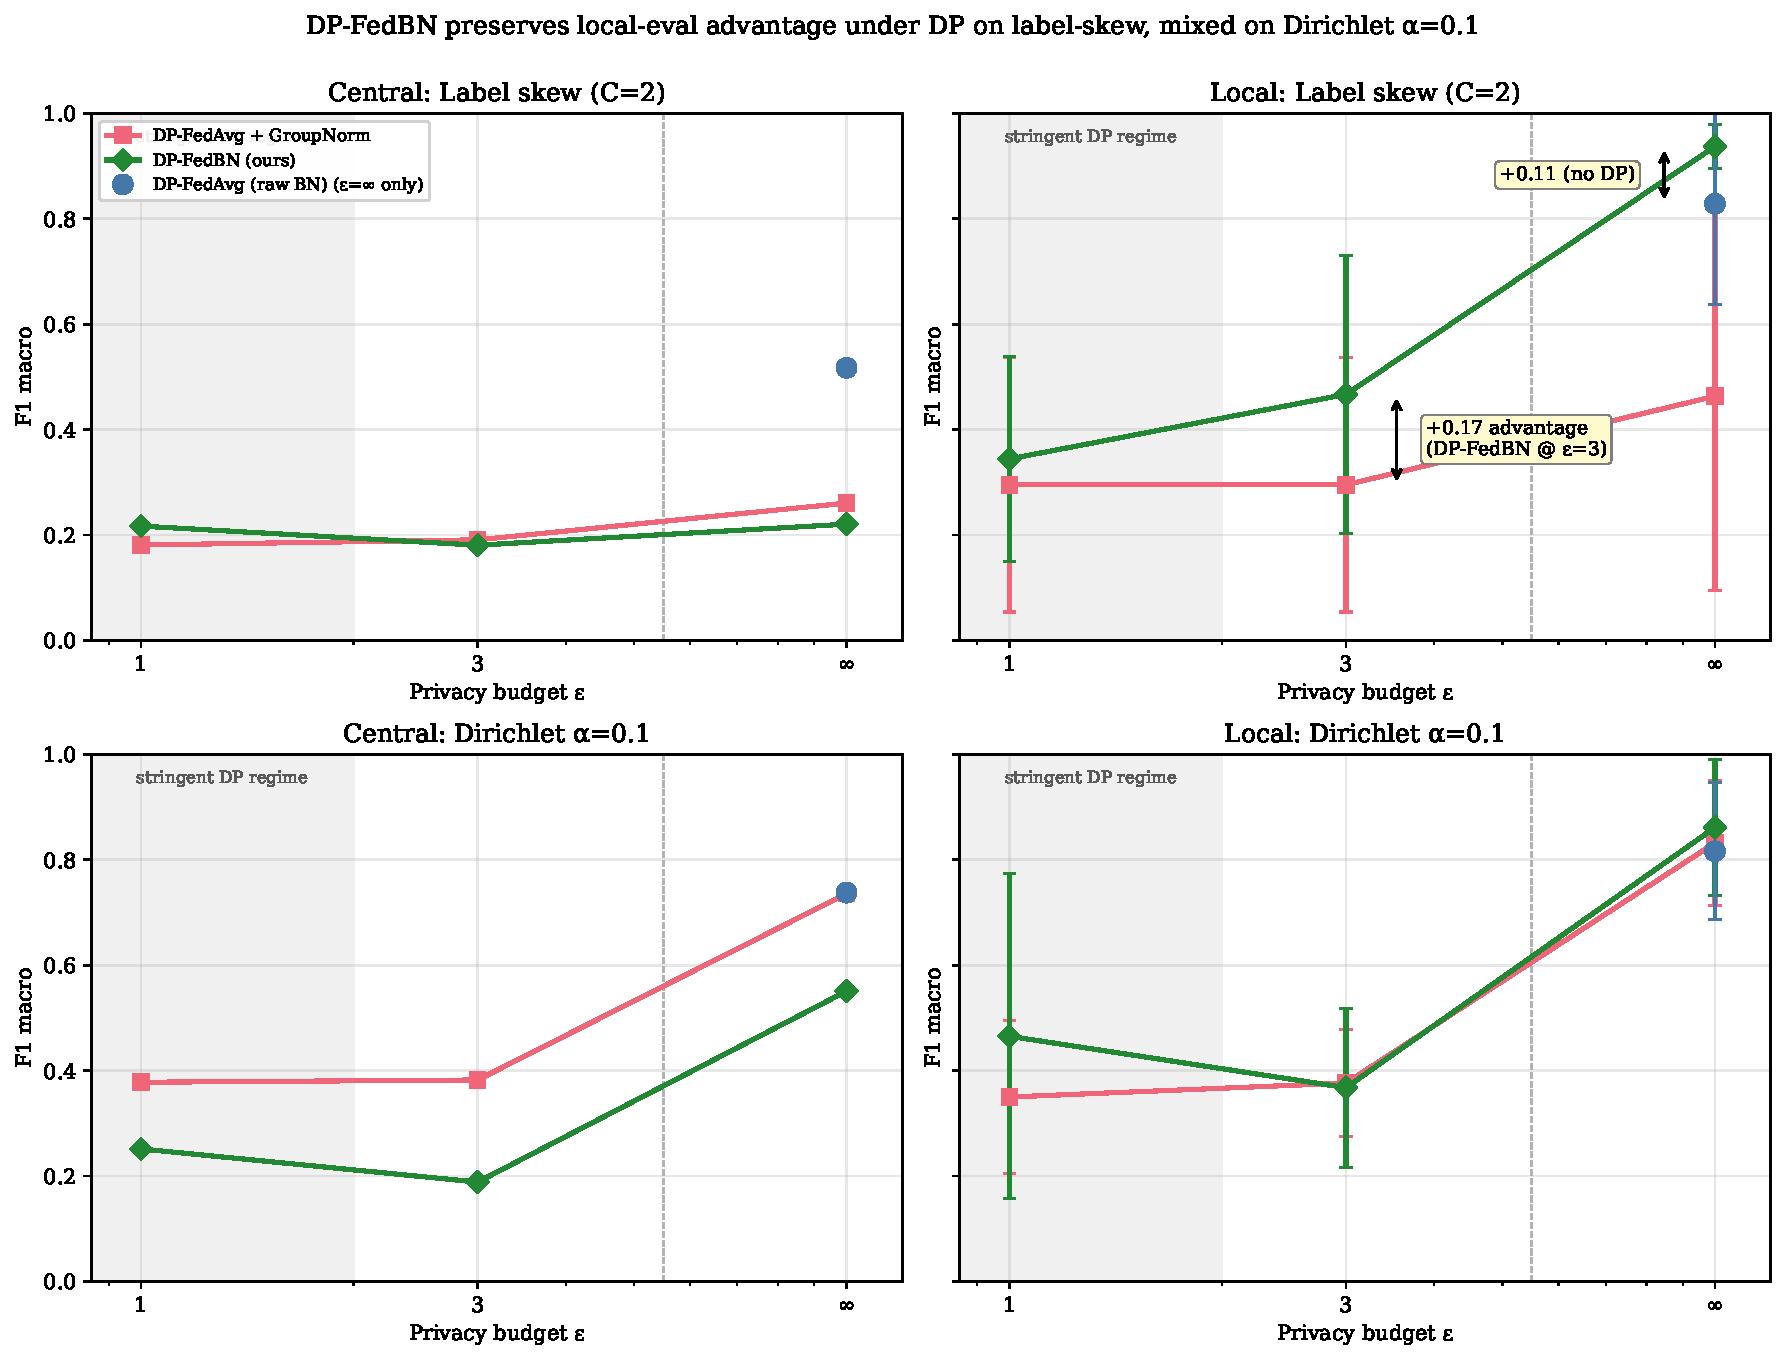
\includegraphics[width=\columnwidth]{fig_privacy_utility.pdf}
\caption{Privacy-utility frontier on MIT-BIH. Top row: label skew $C{=}2$; bottom row: Dirichlet $\alpha{=}0.1$. Left column: central F1; right column: local F1 (mean across 5 clients, shaded $\pm1$ std). DP-FedBN (green) preserves a clear local edge on label skew at $\varepsilon{=}3$; on Dirichlet the edge is mixed.}
\label{fig:dp}
\end{figure}

\emph{Naive DP-FedAvg is empirically refused.} Four of the 18 runs refused at finite $\varepsilon$ (raw BN $\times$ both partitions $\times \{1,3\}$). Opacus's \code{ModuleValidator} cannot be talked into accepting BN with unmodified DP-SGD. This is not an omission --- it is the empirical fact that motivates a non-naive composition like DP-FedBN or the GroupNorm fix.

\emph{On label skew, DP-FedBN preserves a clear local edge.} At $\varepsilon{=}3$, DP-FedBN's local F1 is 0.467 versus 0.295 for DP-FedAvg+GN --- a $+0.17$ gap that survives DP. At $\varepsilon{=}1$ (stringent), the gap shrinks to $+0.05$ but remains positive. At $\varepsilon{=}\infty$ (no DP noise) the gap is $+0.47$. FedBN's mechanism transfers under DP on this partition (Fig.~\ref{fig:dp}).

\emph{On Dirichlet, the local edge is mixed.} At $\varepsilon{=}3$, DP-FedBN local 0.368 versus DP-FedAvg+GN 0.376 --- effectively tied (within plausible single-seed noise). At $\varepsilon{=}1$, DP-FedBN wins again (0.465 vs.\ 0.350, $+0.115$); at $\varepsilon{=}\infty$, DP-FedBN wins by 0.029. The non-monotonicity in $\varepsilon$ is a single-seed signature; we do not over-claim from it.

\subsection{Phase 4: Cross-task replication on PTB-XL}
To strengthen the eval-regime claim from ``MIT-BIH-specific phenomenon'' to ``task-agnostic FL phenomenon,'' we replicate the non-DP and DP sweeps on PTB-XL binary record classification --- a different task (10-second records vs.\ 250-sample beats), different sampling rate (100\,Hz vs.\ 360\,Hz), different number of classes (2 vs.\ 5).

\emph{Non-DP cross-task: eval-regime flip confirmed.} Table~\ref{tab:ptbxl} reports the 12 non-DP runs across 3 partitions $\times$ 4 aggregations. On Dirichlet $\alpha{=}0.1$, FedBN central F1 (0.688) is the lowest of the four aggregations --- and FedBN local F1 (0.588) beats FedAvg local (0.464) by $+0.123$, a larger absolute margin than the same comparison on MIT-BIH Dirichlet ($+0.017$). The eval-regime flip survives a complete change of task (Fig.~\ref{fig:crosstask}).

\begin{table}[t]
\centering
\caption{PTB-XL binary, non-DP cross-task replication. On Dirichlet $\alpha{=}0.1$, the eval-regime flip in FedBN vs.\ FedAvg is preserved: central F1 \emph{below} FedAvg, local F1 \emph{above}.}
\label{tab:ptbxl}
\begin{tabular}{llcc}
\toprule
Partition & Aggregation & Central F1 & Local F1 (mean$\pm$std) \\
\midrule
\multirow{4}{*}{IID} & FedAvg & 0.806 & $0.817 \pm 0.008$ \\
 & FedProx & 0.811 & $0.800 \pm 0.007$ \\
 & FedBN & 0.797 & $0.691 \pm 0.131$ \\
 & FedPerf & 0.812 & $0.789 \pm 0.008$ \\
\midrule
\multirow{4}{*}{Dir.\ $\alpha{=}0.1$} & FedAvg & \textbf{0.804} & $0.464 \pm 0.148$ \\
 & FedProx & 0.817 & $0.661 \pm 0.113$ \\
 & FedBN & 0.688 & $\mathbf{0.588 \pm 0.103}$ \\
 & FedPerf & 0.805 & $0.419 \pm 0.234$ \\
\midrule
\multirow{4}{*}{Lbl.\ $C{=}1^\dagger$} & FedAvg & 0.363 & $0.400 \pm 0.490$ \\
 & FedProx & 0.389 & $0.431 \pm 0.363$ \\
 & FedBN & 0.326 & $1.000 \pm 0.000$ \\
 & FedPerf & 0.397 & $0.462 \pm 0.301$ \\
\bottomrule
\end{tabular}
\\[2pt]
{\footnotesize $^\dagger$ On a binary task, label skew $C{=}1$ gives every client exactly one class; FedBN local F1 is trivially 1.000 (each client predicts its only class perfectly on its own single-class slice). We document the result as a partition design flaw, not a finding.}
\end{table}

\begin{figure*}[t]
\centering
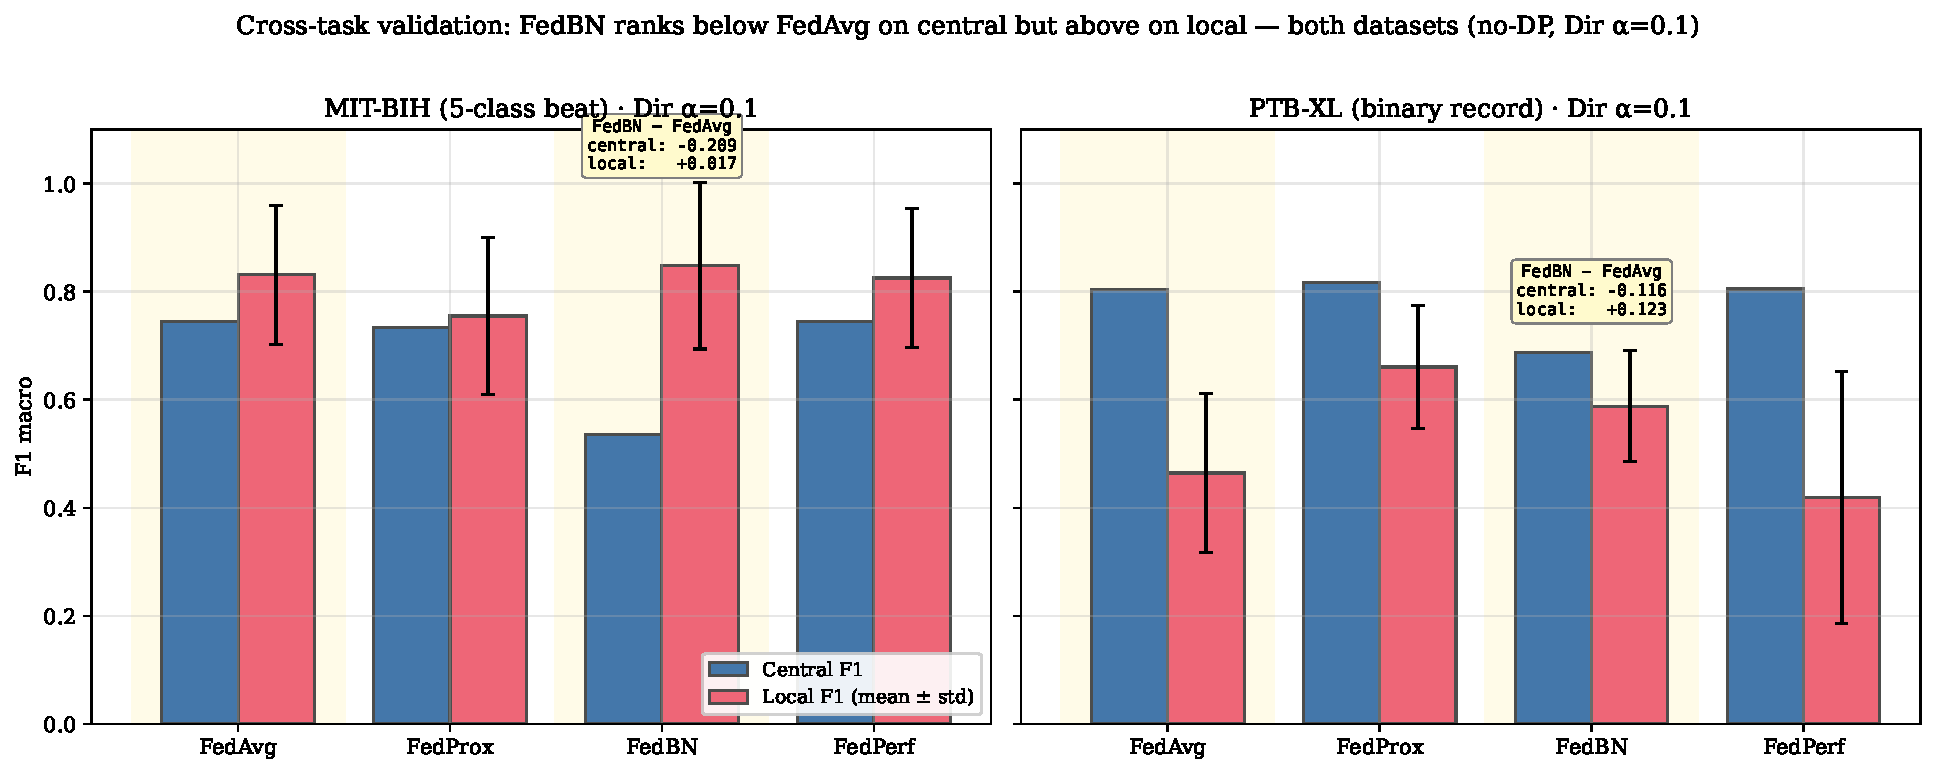
\includegraphics[width=0.95\textwidth]{fig_cross_task.pdf}
\caption{Cross-task summary (Dirichlet $\alpha{=}0.1$, no DP). Both datasets show FedBN central F1 (blue) \emph{below} FedAvg and FedBN local F1 (red) \emph{above} FedAvg. The eval-regime flip in FedBN$-$FedAvg is task-agnostic: $-0.209$ central / $+0.017$ local on MIT-BIH, $-0.116$ central / $+0.123$ local on PTB-XL.}
\label{fig:crosstask}
\end{figure*}

\emph{The label-skew $C{=}1$ partition design flaw.} PTB-XL with \code{classes\_per\_client=1} assigns every client exactly one class (Normal or Abnormal). The trivial signature is FedBN local F1 = 1.0000 with std 0.0000 at every $\varepsilon$ including $\infty$ --- each client's local model predicts its single class correctly on its own slice. The result is invariant to method, partition, or DP noise; it is a partition design flaw on binary tasks, not an algorithmic finding. We exclude it from any DP-FedBN claim.

\emph{DP cross-task: DP-FedBN loses on PTB-XL Dirichlet.} Table~\ref{tab:ptbxldp} reports the 9-cell DP sweep on PTB-XL Dirichlet $\alpha{=}0.1$ (the meaningful partition). At $\varepsilon{=}\infty$, DP-FedBN local (0.604) beats DP-FedAvg+GN (0.443) by $+0.161$, preserving the non-DP rank flip when DP infrastructure is plumbed but no noise is added. At finite $\varepsilon$, the ordering reverses: DP-FedAvg+GN local at $\varepsilon{=}3$ is 0.669 vs.\ DP-FedBN 0.435, a $-0.234$ loss for DP-FedBN. At $\varepsilon{=}1$ the ordering remains: DP-FedAvg+GN 0.715 vs.\ DP-FedBN 0.526 ($-0.189$).

\begin{table}[t]
\centering
\caption{PTB-XL Dirichlet $\alpha{=}0.1$ DP cross-task. DP-FedBN loses to DP-FedAvg+GN at \emph{both} finite $\varepsilon$ values. The non-DP rank flip is preserved at $\varepsilon{=}\infty$ but destroyed by DP noise.}
\label{tab:ptbxldp}
\begin{tabular}{lccc}
\toprule
Method & $\varepsilon$ & Central F1 & Local F1 (mean$\pm$std) \\
\midrule
DP-FedAvg (raw BN) & $\infty$ & 0.807 & $0.552 \pm 0.162$ \\
DP-FedAvg (raw BN) & 3 & \multicolumn{2}{c}{REFUSED} \\
DP-FedAvg (raw BN) & 1 & \multicolumn{2}{c}{REFUSED} \\
DP-FedAvg+GN & $\infty$ & 0.784 & $0.443 \pm 0.142$ \\
DP-FedAvg+GN & 3 & 0.774 & $\mathbf{0.669 \pm 0.109}$ \\
DP-FedAvg+GN & 1 & 0.765 & $\mathbf{0.715 \pm 0.148}$ \\
\textbf{DP-FedBN} & $\infty$ & 0.688 & $0.604 \pm 0.125$ \\
\textbf{DP-FedBN} & 3 & 0.400 & $0.435 \pm 0.054$ \\
\textbf{DP-FedBN} & 1 & 0.451 & $0.526 \pm 0.146$ \\
\bottomrule
\end{tabular}
\end{table}

\emph{Synthesis.} Combining the MIT-BIH and PTB-XL DP results, \textbf{DP-FedBN's local advantage is partition-dependent}:
\begin{itemize}
\item Label skew with $\geq 3$ classes per task (MIT-BIH $C{=}2$): $+0.17$ at $\varepsilon{=}3$. DP-FedBN wins.
\item Dirichlet $\alpha{=}0.1$: tied or losing under DP. MIT-BIH: $-0.008$ at $\varepsilon{=}3$. PTB-XL: $-0.234$ at $\varepsilon{=}3$, the same sign in a sharper magnitude.
\end{itemize}

\section{Discussion}\label{sec:discussion}

\subsection{Why is DP-FedBN's edge partition-dependent?}
FedBN's design choice --- keep client-specific BN running statistics local, never average across clients --- is what gives FedBN its no-DP local advantage. Each client's BN adapts to its own data distribution. In a heterogeneous regime the per-client BN is a \emph{better} normalization for that client's data than any global BN could be.

Under DP, however, the gradients applied to each client's BN parameters\footnote{The BN running statistics $\mu, \sigma^2$ are exponential moving averages, not optimized parameters; they receive no DP noise directly. The BN scale and shift $\gamma, \beta$ are optimized by the plain (non-DP) optimizer \code{opt$_B$} --- they are not noised either. The DP noise enters indirectly: it disturbs the non-BN gradients but indirectly disturbs BN behavior because the noised non-BN updates change the activation statistics that feed the BN running buffers.} are disturbed by DP-driven changes in upstream activations. There is no averaging across clients to smooth the resulting drift --- that averaging is precisely what FedBN avoids. Each client's BN therefore drifts in directions driven more by upstream noise than by data structure, losing its specialization advantage. GroupNorm has no learnable running statistics; the DP noise applied to its affine parameters $(\gamma, \beta)$ \emph{is} averaged across clients during aggregation, damping it.

\emph{Why label skew differs from Dirichlet.} On label skew $C{=}2$ each client owns only 2 of 5 classes; the specialization FedBN's per-client BN provides is so much better than a globally-averaged BN that even noised FedBN local performance beats GroupNorm local at $\varepsilon{=}3$ (Table~\ref{tab:dp}). Specialization wins over averaging when specialization-distance is large. On Dirichlet $\alpha{=}0.1$ each client has skewed-but-not-truncated class proportions; DP noise costs more than it gains, and GroupNorm wins. Specialization-distance is small; a globally-averaged BN is a reasonable normalizer for any client, and the magnitude depends on how much specialization is available to lose.

\subsection{Practitioner rubric}
The findings translate to a small decision rubric for medical FL practitioners. (i)~\emph{Label-truncated heterogeneity} (specialty hospitals, single-condition clinics): DP-FedBN preserves a clear local-F1 edge under DP and the dual-optimizer overhead is justified. (ii)~\emph{Proportional heterogeneity} (general hospitals with mixed case-mix): DP-FedAvg+GroupNorm is simpler and at least as good --- often better. (iii)~\emph{Local deployment priority} (each site uses its own personalized model): FedBN (no DP) gives the strongest local F1; if DP is required, DP-FedBN is competitive on label-truncated data and competitive-or-worse on proportional data. (iv)~\emph{Strict regulatory pooled-central requirements}: FedAvg or FedPerf, not FedBN --- the eval-regime flip means FedBN's central F1 ranks worst even when its local F1 ranks best.

\subsection{The eval-regime choice is methodological}
A reader who reports ``central F1 on a held-out test pool'' as the primary metric will see FedBN underperforming. The same reader evaluating per-client may see FedBN winning. Whether to report central or local F1 is not a stylistic choice --- \emph{it changes the conclusion}. We argue both regimes should be reported when the deployment scenario is itself ambiguous between them. Most FL benchmarking papers, including the original FedBN~\cite{fedbn}, report only one regime; we suggest this is a missing variable.

\section{Conclusion}\label{sec:conclusion}
We presented DP-FedBN, a dual-optimizer composition of DP-SGD with FedBN that preserves per-client BatchNorm specialization while applying DP to the parameters that actually cross the federation boundary. Across two medical ECG datasets, six non-IID partition regimes, and three privacy budgets, three findings emerge.

\emph{First}, the eval-regime flip FedBN induces under label heterogeneity is task-agnostic: FedBN underperforms in pooled-central evaluation while overperforming in per-client local evaluation, on both MIT-BIH 5-class beats and PTB-XL binary records. The choice between central and local evaluation matters more than the choice between aggregation methods in many realistic deployment scenarios.

\emph{Second}, DP-FedBN's local advantage under DP is partition-dependent: $+0.17$ at $\varepsilon{=}3$ on MIT-BIH label-skew $C{=}2$ (DP-FedBN wins), but $-0.008$ on MIT-BIH Dirichlet and $-0.234$ on PTB-XL Dirichlet at the same budget (DP-FedAvg+GN wins). The mechanism --- DP-driven activation noise propagating to per-client BN parameters without cross-client averaging --- is consistent with this sign across both datasets.

\emph{Third}, naive DP-FedAvg on a BN-containing model is empirically refused by Opacus's \code{ModuleValidator} at finite $\varepsilon$, which is the empirical motivation for the dual-optimizer formulation rather than a side observation.

\emph{Practical guidance.} Use DP-FedBN when sites are label-truncated (specialty clinics, single-condition cohorts) and local deployment is the goal; use DP-FedAvg+GroupNorm when sites have proportional class-mix heterogeneity. Report both central and local F1 when the deployment regime is itself ambiguous.

\emph{Limitations.} All results are single-seed (\code{seed=42}); multi-seed expansion is the most important deferred experiment. The CNN1D architecture is fixed; heterogeneity is simulated on pooled datasets, not measured cross-institutionally; client count is 5 (production FL has dozens to hundreds); validation is ECG-only. FedProx runs use $\mu{=}0.01$ and likely under-perform due to insufficient hyperparameter tuning. Multi-label PTB-XL with all 12 leads (macro-AUC over 5 superclasses) is the natural follow-up.

\emph{Reproducibility.} All code, configurations, and per-run logs are at \url{https://github.com/kanemoda/MedicalFL} (private during review, public upon acceptance). Seed 42; cuDNN deterministic with benchmark on; Opacus 1.5; PyTorch 2.4.

\section*{Acknowledgments}
LLM-assisted tooling (a coding agent and a deep-research literature scanner) was used during implementation and literature review; all experimental decisions, results, and final paper text are the authors' own. Computational resources were provided by Ege University.

\begin{thebibliography}{00}
\bibitem{adcol} Q.~Li, B.~He, and D.~Song, ``Adversarial collaborative learning on non-IID features,'' in \emph{Proc.\ 40th Int.\ Conf.\ Machine Learning (ICML)}, ser.\ PMLR, vol.~202, 2023, pp.\ 19504--19526.
\bibitem{fedavg} B.~McMahan, E.~Moore, D.~Ramage, S.~Hampson, and B.~Ag\"{u}era y Arcas, ``Communication-efficient learning of deep networks from decentralized data,'' in \emph{Proc.\ 20th Int.\ Conf.\ Artificial Intelligence and Statistics (AISTATS)}, ser.\ PMLR, vol.~54, 2017, pp.\ 1273--1282.
\bibitem{rieke} N.~Rieke, J.~Hancox, W.~Li, F.~Milletar\`{i}, H.~R.~Roth, S.~Albarqouni, S.~Bakas, M.~N.~Galtier, B.~A.~Landman, K.~Maier-Hein, \emph{et al.}, ``The future of digital health with federated learning,'' \emph{npj Digital Medicine}, vol.~3, no.~1, p.~119, 2020.
\bibitem{geyer} R.~C.~Geyer, T.~Klein, and M.~Nabi, ``Differentially private federated learning: A client level perspective,'' in \emph{NeurIPS Workshop on Machine Learning on the Phone and other Consumer Devices}, 2017.
\bibitem{abadi} M.~Abadi, A.~Chu, I.~Goodfellow, H.~B.~McMahan, I.~Mironov, K.~Talwar, and L.~Zhang, ``Deep learning with differential privacy,'' in \emph{Proc.\ 2016 ACM SIGSAC Conf.\ Computer and Communications Security (CCS)}, 2016, pp.\ 308--318.
\bibitem{batchnorm} S.~Ioffe and C.~Szegedy, ``Batch normalization: Accelerating deep network training by reducing internal covariate shift,'' in \emph{Proc.\ 32nd Int.\ Conf.\ Machine Learning (ICML)}, ser.\ PMLR, vol.~37, 2015, pp.\ 448--456.
\bibitem{opacus} A.~Yousefpour, I.~Shilov, A.~Sablayrolles, D.~Testuggine, K.~Prasad, M.~Malek, J.~Nguyen, S.~Ghosh, A.~Bharadwaj, J.~Zhao, G.~Cormode, and I.~Mironov, ``Opacus: User-friendly differential privacy library in PyTorch,'' \emph{arXiv preprint arXiv:2109.12298}, 2021.
\bibitem{groupnorm} Y.~Wu and K.~He, ``Group normalization,'' in \emph{Proc.\ European Conf.\ Computer Vision (ECCV)}, ser.\ LNCS, vol.~11217.\ Springer, 2018, pp.\ 3--19.
\bibitem{fedbn} X.~Li, M.~Jiang, X.~Zhang, M.~Kamp, and Q.~Dou, ``FedBN: Federated learning on non-IID features via local batch normalization,'' in \emph{Int.\ Conf.\ Learning Representations (ICLR)}, 2021.
\bibitem{opacusissue} Opacus contributors, ``Allow batchnorm layers with frozen running stats (issue \#472),'' GitHub, 2022. [Online]. Available: \url{https://github.com/pytorch/opacus/issues/472}
\bibitem{fedprox} T.~Li, A.~K.~Sahu, M.~Zaheer, M.~Sanjabi, A.~Talwalkar, and V.~Smith, ``Federated optimization in heterogeneous networks,'' in \emph{Proc.\ Machine Learning and Systems (MLSys)}, vol.~2, 2020, pp.\ 429--450.
\bibitem{tia} J.~Tia, L.~Meng, S.~Li, J.~Liu, and D.~Wu, ``Federated motor imagery classification for privacy-preserving brain-computer interfaces,'' 2024.
\bibitem{privatefl} Y.~Yang, B.~Hui, H.~Yuan, N.~Gong, and Y.~Cao, ``PrivateFL: Accurate, differentially private federated learning via personalized data transformation,'' in \emph{32nd USENIX Security Symposium}, 2023, pp.\ 1595--1612.
\bibitem{resnetfed} P.~Riedel, R.~von Schwerin, D.~Schaudt, A.~Hafner, and C.~Sp\"{a}te, ``ResNetFed: Federated deep learning architecture for privacy-preserving pneumonia detection from COVID-19 chest radiographs,'' \emph{Journal of Healthcare Informatics Research}, vol.~7, no.~2, pp.\ 203--224, 2023.
\bibitem{fedonco} V.~C.~Marella, S.~R.~Veluru, and S.~T.~Erukude, ``FedOnco-Bench: A reproducible benchmark for privacy-aware federated tumor segmentation with synthetic CT data,'' 2025.
\bibitem{kairouz} P.~Kairouz, H.~B.~McMahan, B.~Avent, A.~Bellet, M.~Bennis, A.~N.~Bhagoji, K.~Bonawitz, Z.~Charles, G.~Cormode, R.~Cummings, \emph{et al.}, ``Advances and open problems in federated learning,'' \emph{Foundations and Trends in Machine Learning}, vol.~14, no.~1--2, pp.\ 1--210, 2021.
\bibitem{adamw} I.~Loshchilov and F.~Hutter, ``Decoupled weight decay regularization,'' in \emph{Int.\ Conf.\ Learning Representations (ICLR)}, 2019.
\bibitem{mitbih} G.~B.~Moody and R.~G.~Mark, ``The impact of the MIT-BIH arrhythmia database,'' \emph{IEEE Engineering in Medicine and Biology Magazine}, vol.~20, no.~3, pp.\ 45--50, 2001.
\bibitem{ec57} ANSI/AAMI, ``Testing and reporting performance results of cardiac rhythm and ST segment measurement algorithms,'' ANSI/AAMI EC57:2012(R)2020, 2012.
\bibitem{dechazal} P.~de Chazal, M.~O'Dwyer, and R.~B.~Reilly, ``Automatic classification of heartbeats using ECG morphology and heartbeat interval features,'' \emph{IEEE Trans.\ Biomedical Engineering}, vol.~51, no.~7, pp.\ 1196--1206, 2004.
\bibitem{mondejar} V.~Mond\'{e}jar-Guerra, J.~Novo, J.~Rouco, M.~G.~Penedo, and M.~Ortega, ``Heartbeat classification fusing temporal and morphological information of ECGs via ensemble of classifiers,'' \emph{Biomedical Signal Processing and Control}, vol.~47, pp.\ 41--48, 2019.
\bibitem{ptbxl} P.~Wagner, N.~Strodthoff, R.-D.~Bousseljot, D.~Kreiselmeier, F.~I.~Lunze, W.~Samek, and T.~Schaeffter, ``PTB-XL, a large publicly available electrocardiography dataset,'' \emph{Scientific Data}, vol.~7, no.~1, p.~154, 2020.
\end{thebibliography}

\end{document}
